\documentclass[a4paper,10pt, notitlepage]{report}
\usepackage[utf8]{inputenc}
\usepackage{natbib}
\usepackage{amssymb}
\usepackage{subfig}
\usepackage{amsmath}
\usepackage{enumitem}
\usepackage{graphicx}
\usepackage[portuguese]{babel}
\usepackage{amsmath}%
%\usepackage[square,sort,comma,numbers]{natbib}
\usepackage{graphics}
\usepackage{booktabs} 
%\usepackage{MnSymbol}%
\usepackage{stackrel}
%\usepackage{wasysym}%

\newtheorem{defi}{Definicão}
\newtheorem{teo}{Teorema}
\newtheorem{col}{Corolário}
\setlength{\parindent}{0em}
\newcommand{\indep}{\perp \!\!\! \perp} %% indepence
\newcommand{\gt}{>}%broken keyboard
\newcommand{\pow}{^}%broken keyboard
\newcommand{\pr}{\operatorname{Pr}} %% probability
\newcommand{\vr}{\operatorname{Var}} %% variance
\newcommand{\rs}{X_1, X_2, \ldots, X_n} %%  random sample
\newcommand{\irs}{X_1, X_2, \ldots} %% infinite random sample
\newcommand{\rsd}{x_1, x_2, \ldots, x_n} %%  random sample, realised
\newcommand{\Sm}{\bar{X}_n} %%  sample mean, random variable
\newcommand{\sm}{\bar{x}_n} %%  sample mean, realised
\newcommand{\Sv}{\bar{S}^2_n} %%  sample variance, random variable
\newcommand{\sv}{\bar{s}^2_n} %%  sample variance, realised
\newcommand{\bX}{\boldsymbol{X}} %%  random sample, contracted form (bold)
\newcommand{\bx}{\boldsymbol{x}} %%  random sample, realised, contracted form (bold)
\newcommand{\bT}{\boldsymbol{T}} %%  Statistic, vector form (bold)
\newcommand{\bt}{\boldsymbol{t}} %%  Statistic, realised, vector form (bold)
\newcommand{\emv}{\hat{\theta}_{\text{EMV}}}
\newcommand{\defn}{\stackrel{\textrm{\scriptsize def}}{=}}
\newcommand{\mysection}[2]{\setcounter{section}{#1}\addtocounter{section}{-1}\section*{#1 - #2}}
\newcommand{\op}{\operatorname}

% Title Page
\title{Trabalho IV: Testes uniformemente mais poderosos.}
\author{Disciplina: Inferência Estatística \\ Aluno: Rener de Souza Oliveira}

\begin{document}
	\maketitle

	
	\section*{Introdução}
	
	Vimos que os testes de hipótese fornecem uma abordagem matematicamente sólida para traduzir hipóteses científicas sobre o processo gerador dos dados em decisões sobre os dados -- isto é, traduzir afirmações sobre partições do espaço de parâmetros, $\Omega$, em afirmações testáveis sobre o espaço amostral $\mathcal{X}^n$.
	
	Um teste $\delta(\bX)$ é uma decisão (binária) de rejeitar ou não uma hipótese nula ($H_0$) sobre $\theta \in \Omega$ com base em uma amostra $\bX$.
	A capacidade de um teste de rejeitar $H_0$ quando ela é falsa é medida pela função poder, $\pi(\theta |\delta)$.
	Nem todos os testes, no entanto, são criados iguais.
	Em certas situações, é possível mostrar que um procedimento $\delta_A$ é~\textit{uniformemente} mais poderoso que outro procedimento $\delta_B$ para testar a mesma hipótese.
	
	Neste trabalho, vamos definir e aplicar o conceito de~\textbf{teste uniformemente mais poderoso}.
	
	\mysection{1}{Motivação e Definição}
	
	Sejam:
	
	\begin{align}
	\label{h0h1}
	 H_0:& \theta \in \Omega_0\subset \Omega,\nonumber\\
	 H_1:& \theta \in \Omega_1\subset \Omega,\\
	 \text{onde } &\Omega_1= \Omega \setminus \Omega_0\nonumber
	\end{align}
	
	%De tal forma que $H_1$ seja composta, ou seja, possui cardinalidade maior que 1.
	
	Ao realizar um procedimento de teste $\delta(\bX)$, é desejável que a função poder $\pi(\theta|\delta):\defn \op{Pr}(Rejeitar ~H_0|\theta)$ seja menor ou igual à um nível de significância $\alpha_0\in (0,1)$, quando $\theta\in\Omega_0$, limitando superiormente a probabilidade de erro do tipo I (rejeitar $H_0$ quando ela é verdadeira). Podemos expressar tal propriedade da seguinte forma:
	
	\begin{align*}
		\alpha(\delta)\leq \alpha_0
	\end{align*}
	
	Onde $\displaystyle\alpha(\delta):\defn\sup_{\theta\in\Omega_0}\pi(\theta|\delta)$ é o tamanho do teste.
	
	
	
	Além disso, queremos também ter algum controle sobre a probabilidade de erro do tipo II (não rejeitar $H_0$ quando ela é falsa). Como a probabilidade de tal erro quando $\theta \in \Omega_1$ é igual a $1-\pi(\theta|\delta)$, queremos que, na região onde $H_0$ é falsa ($\Omega_1$) a função poder $\pi(\theta|\delta)$ seja máxima, para todo $\theta$ em tal região. Tal maximização, minimiza a probabilidade de erro do tipo II quando $\theta\in\Omega_1$, isso nem sempre é possível, mas quando for, temos um nome especial para esse teste, que segue abaixo sua definição:
	
	\begin{defi}
		\textbf{(Teste Uniformemente mais poderoso)}
		\label{ump} 
		Seja $\mathcal{C}$ uma classe de teste para as hipóteses (\ref{h0h1}); $\delta^*\in\mathcal{C}$ é chamado de uniformemente mais poderoso (UMP\footnote{Uniformly Most Powerful Test}) da classe $\mathcal{C}$, se:
		
		\begin{align*}\pi(\theta|\delta^*)&\geq\pi(\theta|\delta) ~\forall \,\theta \in \Omega_1,
		\end{align*}
		
		para qualquer teste $\delta\in\mathcal{C}$.
		
	\end{defi} 
	Seguindo a motivação dada acima, podemos definir $\mathcal{C}$ como o conjunto de todos dos testes de tamanho menor ou igual a $\alpha_0$, limitando o erro tipo I. Neste caso, chamamos $\delta^*$ de UMP para (\ref{h0h1}) ao nível $\alpha_0$.
	
	\mysection{2}{Razão de Verossimilhança Monótona}
	
	\begin{defi}
		\textbf{(Razão de Verossimilhanças Monótona)} Seja $f_n(\bx|\theta)$ a função de verossimilhança das observações $\bX = (\rs)$, e $T=r(\bX)$ uma estatística. Dizemos que a distribuição dos dados tem \textbf{razão de verossimilhanças monótona} sob $T$, quando, $\forall\,\theta_1,\theta_2\in\Omega; \theta_1<\theta_2$, a razão $\dfrac{f(\bx|\theta_2)}{f(\bx|\theta_1)}$ depende dos dados através de $r(\bx)$ somente, e é uma função monótona de $r(\bx)$ sob seu espaço de definição.
	\end{defi}

	\mysection{3}{UMP para $H_0$ simples}
	
	Considere uma hipótese nula simples, $H_0: \theta = \theta_0$, $\theta_0 \in \Omega$.
	Mostraremos que, se vale o Teorema da Fatorização, e existem $c$ e $\alpha_0$ tais que
	\begin{equation}
	\pr\left(r(\bX) \geq c \mid \theta = \theta_0\right) = \alpha_0\nonumber,
	\end{equation}
	então o procedimento $\delta^\ast$ que rejeita $H_0$ se $r(\bX) \geq c$ é UMP para $H_0$ ao nível $\alpha_0$.
	
	Mas antes, vamos enunciar alguns teoremas:
	
	\begin{teo}
		\textbf{(Teorema da Fatorização)\citep{degroot2012probability_fact}}
		Sejam $\rs$ amostra aleatória de uma distribuição de densidade ou massa $f(x|\theta)$, onde $\theta\in\Omega$. Uma estatística $T=r(\rs)$ é suficiente para $\theta$, se, e somente se a distribuição conjunta dos dados $f_n(\bx|\theta)$ pode ser fatorizada como:
		
		\begin{align*}
			f_n(\bx|\theta) = u(\bx)v[r(\bx),\theta],
		\end{align*}
		
		para todo $\bx= (\rsd)\in\mathbb{R}^n$, e $\forall \theta \in \Omega$. $u$ e $v$ são funções não negativas.
		
	\end{teo}

	A demostração pode ser encontrada em \citep{degroot2012probability_fact}.
	
	\begin{teo}
		\textbf{(Lema de Neyman-Pearson)\citep{CaseBerg:01}} Seja $(\rs)\in\mathbb{R}^n$ uma amostra indexada por $\theta$. Considere as hipóteses
		
		\begin{align}
		\label{hnp}
		H_0:\theta=\theta_0,\\
		H_1:\theta=\theta_1,\nonumber
		\end{align}
		
		e seja $f_n(\bx|\theta_i)$, com $i=0,1$ a função de densidade ou massa dos dados.
		
		Seja $R\in\mathbb{R}^n$ uma região de rejeição que satisfaça:
		
		\begin{align}
		\label{np1}
			\bx\in R\text{ se } f(\bx|\theta_1)\geq kf(\bx|\theta_0)\nonumber\\ \\\text{ e }\bx\in R^C\text{ se } f(\bx|\theta_1)\leq k f(\bx|\theta_0),\nonumber
		\end{align}
		
		para algum $k\geq0$ e 
		
		\begin{align}
		\label{np2}
			\pr(\bX\in R|\theta = \theta_0)=\alpha_0.
		\end{align}
		
		Então, todo teste que satisfaz (\ref{np1}) e (\ref{np2}) é UMP ao nivel $\alpha_0$.
	\end{teo}

	A demostração será omitida pois pode ser encontrada em \citep{CaseBerg:01}.
	
	\begin{col}
		\label{colnp}
		Considere as hipóteses (\ref{hnp}). Seja $T(\bX)$ uma estatística suficiente para $\theta$ e $g(t|\theta_i)\,i=0,1$, uma função de $t=T(\bx)$ tal que fatoriza a verossimilhança dos dados em $f_n(\bx|\theta_i)=g(t|\theta_i)u(\bx)$, para alguma função $u(\bx)\geq0$.
		
		Seja $\delta$ um teste que rejeite $H_0$ se $T$ pertence a uma região de rejeição $S$ (subconjunto do espaço de definição de $T$). Assim, $\delta$ será UMP ao nível $\alpha_0$ se satisfazer:
		
		\begin{align}
		\label{col1}
		 g(t|\theta_1)\geq  kg(t|\theta_0)\implies t\in S\nonumber\\ \\\text{ e }g(t|\theta_1)\leq kg(t|\theta_0)\implies t\in S\pow C,\nonumber
		\end{align}
		
		para algum $k\geq0$ e 
		
		\begin{align}
		\label{col2}
		\pr[T(\bX)\in S|\theta = \theta_0]=\alpha_0.
		\end{align}
		
	\end{col}
	\textbf{Demonstração:} Definindo $R=\{\bx|T(\bx)\in S\}$, rejeitaremos $H_0$ se $\bx \in R$. Pelo Teorema da Fatorização, dado que $T(\bX)$ é suficiente, a verossimilhança de $\bX$ pode ser escrita como $f_n(\bx|\theta_i)=g(T(\bx)|\theta_i)u(\bx),\,i=0,1$, para alguma função $u(\bx)\geq 0$.
	
	Multiplicando tal função nas desigualdades (\ref{col1}) temos:
	
	\begin{align*}
		&g(T(\bx)|\theta_1)\geq kg(T(\bx)|\theta_0)\\
		\Leftrightarrow&
		g(T(\bx)|\theta_1)u(\bx)\geq kg(T(\bx)|\theta_0)u(\bx)\\
		\Leftrightarrow&f_n(\bx|\theta_1)\geq kf_n(\bx|\theta_0)
	\end{align*}
	
	Assim, tem-se: $f_n(\bx|\theta_1)\geq kf_n(\bx|\theta_0)\implies T(\bx)\in S\implies \bx \in R$.
	
	Analogamente, $f_n(\bx|\theta_1)\leq kf_n(\bx|\theta_0)\implies \bx \in R\pow C$.
	
	
	De (\ref{col2}), tem-se:
	
	\begin{align*}
		\pr(\bX\in R|\theta=\theta_0)=\pr[T(\bX)\in S|\theta = \theta_0] = \alpha_0	
	\end{align*}
	
	Pelo \textbf{Lema de Neyman-Pearson} concluímos que o teste $\delta$ é UMP ao nível $\alpha_0$.
	
	
	Voltando agora ao problema inicial da seção, queremos provar que $\delta\pow*$ é UMP ao nível $\alpha_0$ para $H_0:\theta=\theta_0$.
	
	Primeiramente precisamos provar que $\alpha(\delta\pow*)=\alpha_0$.
	
	\begin{align*}
	\displaystyle\alpha(\delta\pow*)&=\sup_{\theta\in\Omega_0}\pi(\theta|\delta\pow*)\\
	&=\sup_{\theta\in\Omega_0}\pr[r(\bX)\geq c|\theta]
	\end{align*}
	
	Como $\Omega_0=\{\theta_0\}$, o supremo ocorre em $\theta_0$ o que implica que $\alpha(\delta\pow*)=\alpha_0$.
	
	Agora precisamos provar que $\delta\pow*$ é UMP.
	
	Façamos $\theta'$ arbitrário, com $\theta'\neq \theta_0$, testaremos $H_0:\theta=\theta_0$ contra $H_1':\theta=\theta'$.  No problema em questão, vale o \textbf{Teorema da Fatorização} para $r(\bX)$, logo assumindo sua suficiência, temos que a verossimilhança pode ser escrita como $f_n(\bx|\theta)=g(r(\bx)|\theta)u(\bx)$, para alguma função $u(\bx)\geq0$.
	
	Seja $t=r(\bx)$; Definamos:
	
	\begin{align*}
		k=\inf_{t\in\mathcal{T}}\dfrac{f_n(\bx|\theta')}{f_n(\bx|\theta_0)}=\dfrac{g(t|\theta')}{g(t|\theta_0)}
	\end{align*}
	
	Com $\mathcal{T}:\defn\{t|t\geq c\}$
	
	Tal ínfimo existe, pois pelo Teorema da Fatorização, a função $g$ é não-negativa, logo, o conjunto na qual estamos tomando ínfimo é limitado inferiormente por 0. Pelo análogo do Axioma do Supremo para ínfimos, $k$ está bem definido.
	
	Pela definição de ínfimo segue que:
	
	$r(\bx)\geq c\Leftrightarrow \dfrac{g(r(\bx)|\theta')}{g(r(\bx)|\theta_0)}\geq k$.
	
	Pelo Corolário \ref{colnp} do Lema de Neyman-Pearson, temos que $\delta\pow*$ é UMP para as hipóteses $H_0:\theta=\theta_0$ e $H_1':\theta=\theta'$, ou seja, $\pi(\theta|\delta\pow*)\geq\pi(\theta'|\delta)$, para qualquer teste $\delta$ de tamanho $\alpha_0$. Como $\theta'$ foi escolhido arbitrariamente diferente de $\theta_0$, temos que $\delta\pow*$ satisfaz $\pi(\theta|\delta\pow*)\geq\pi(\theta'|\delta)~\forall\,\theta'\neq\theta_0$, o que prova nossa afirmação inicial. $\blacksquare$
	
	\mysection{4}{Duas-Caras e UMP para Bernoulli}
	
	Suponha que você encontra o Duas-Caras na rua e ele não vai com a sua... cara. 
	Ele decide jogar a sua famosa moeda para o alto para decidir se te dá um cascudo.
	Se der cara ($C$), você toma um cascudo.
	Você, que sabe bem Estatística, pede que ele pelo menos jogue a moeda umas $n=10$ vezes antes de tomar a decisão derradeira.
	
	Surpreendentemente, ele concorda. 
	Lança a moeda e obtém
	$$ \text{KCKCKCCKKK} $$
	
	Você agora deve decidir se foge, se arriscando a tomar dois cascudos ao invés de um, ou se fica e  possivelmente não toma cascudo nenhum.
	Se $p$ é a probabilidade de dar cara, estamos interessados em testar a hipótese
	\begin{align*}
	H_0 &:  p \leq \frac{1}{2},\\
	H_1 &:p > \frac{1}{2}.
	\end{align*}
	
	\begin{enumerate}
		\item Escreva a razão de verossimilhanças para esta situação;
		
		Sejam $p_0$ e $p_1$, tais que $0<p_0\leq \frac{1}{2}<p_1<1$. Seja $X_i$ a variável indicadora de cara no $i$-ésimo lançamento do Duas-Caras; Assumindo que os 10 lançamentos são independentes, temos $X_1,X_2,\ldots,X_{10}\stackrel{iid}{\sim} \op{Bernoulli}(p)$, na qual $f(x_i|p)=p\pow{x_i}(1-p)\pow{1-x_i}$.
		
		A verossimilhança sera então:
		
		$$f_n(\bx|p)=\prod_{i=1}^{10}p\pow{x_i}(1-p)\pow{1-x_i}=p\pow{y}(1-p)\pow{10-y},$$
		
		onde $\displaystyle y=\sum_{i=1}^{10}x_i$.
		
		Assim, a razão de verossimilhança será:
		
		\begin{align}
			\dfrac{f_n(\bx|p_1)}{f_n(\bx|p_0)}&=\dfrac{p_1\pow{y}(1-p_1)\pow{10-y}}{p_0\pow{y}(1-p_0)\pow{10-y}}\nonumber\\
			&=\left[\dfrac{p_1(1-p_0)}{p_0(1-p_1)}\right]\pow y\left(\dfrac{1-p_1}{1-p_0}\right)\pow{10}\label{lik_ratio}
		\end{align}
		
		Podemos ver que a razão depende dos dados somente através da estatística suficiente $y$, e que a expressão é monótona em $y$, pois $p_0<p_1\Rightarrow \dfrac{p_1(1-p_0)}{p_0(1-p_1)}>1$, que mostra que a razão é estritamente crescente neste caso. Por definição, dizemos que a distribuição dos dados tem razão de verossimilhança monótona crescente sob $y$ (MLR\footnote{Monotone Likelihood Ratio} crescente).
		
		%Veja também que a distribuição da estatística $y$ também terá razão de verossimilhança monótona (sob o próprio $y$), pois é soma de 10 variáveis i.i.d bernoulli(p), logo $y\sim \op{Binomial}(10,p)$, cuja verossimilhança se descreve por $\mathcal{L}(p;y)={10\choose´ y}p\pow y (1-p)\pow{10-y}$. Se escolhermos $p_0<p_1$ como antes, a razão $\dfrac{\mathcal{L}(p_1;{y})}{\mathcal{L}(p_0;{y})}$ será exatamente igual a expressão (\ref{lik_ratio}), pois o termo ${10\choose y}$ se cancela. Assim, a distribuição da estatística suficiente $y=\displaystyle\sum_{i=1}^{10}x_i$ também tem MLR crescente.
		
		\item Nesta situação, é do seu interesse encontrar um teste UMP.
		Faça isso e aplique o teste desenvolvido aos dados que conseguiu arrancar do Duas-Caras.
		
		Existe uma generalização dos resultados da seção anterior, que estende a noção de existência de UMP para $H_0$ composta, e inclui a hipótese de distribuição com MLR. Vamos enunciá-lo e demonstrá-lo brevemente, pois basta algumas adaptações da demonstração da seção anterior para $H_0$ simples.
		
		\begin{teo}
			\textbf{(Teorema de Karlin-Rubin)\citep{CaseBerg:karlin}} Sejam as hipóteses:
			
			\begin{align}
			\label{h0_karlin}
				H_0:\theta\leq\theta_0\\
				H_1:\theta\gt\theta_0\nonumber
			\end{align}
			
			Seja $T=r(\bX)$ uma estatística suficiente para $\theta$ e suponha que a família de distribuições dos dados $\{f(\bx|\theta)|\theta\in\Omega\}$ tem razão de verossimilhança monótona não-decrescente sob $T$. Assim, para qualquer $c$, o teste $\delta\pow*$ que rejeita $H_0$ se $T\geq c$ é um teste UMP ao nível $\alpha_0$, onde $\alpha_0=\pr[T\geq c\,|\theta=\theta_0]$.
		\end{teo} 
	
	\textbf{Demonstração:} Devemos mostrar que o tamanho do teste é $\alpha_0$ e que $\delta\pow*$ é UMP. O fluxo da demostração será parecido com a do Corolário (\ref{colnp}).
	
	Para a primeira parte, queremos que,
	
	$$\sup_{\theta\leq\theta_0}\pr[T\geq c\,|\theta]=\alpha_0$$
	
	Na última demostração o supremo era trivial pois era tomado em um conjunto unitário, agora a situação se complica. Se a função poder for não-decrescente, o supremo ocorrerá em $\theta_0$ e fica provada essa parte, pois foi suposto que $\pr[T\geq c\,|\theta=\theta_0]=\alpha_0$. Provaremos isso ao longo deste texto. 
	
	Fixemos $\theta'$ arbitrário tal que $\theta'>\theta_0$, testaremos $H_0':\theta=\theta_0$ contra $H_1':\theta=\theta'$.  Como $T=r(\bX)$ é suficiente, pelo \textbf{Teorema da Fatorização}, temos que a verossimilhança pode ser escrita como $f_n(\bx|\theta)=g(t|\theta)u(\bx)$, para alguma função $u(\bx)\geq0$, com $t=r(\bx)$.
	
	Definamos:
	
	\begin{align*}
	k=\inf_{t\in\mathcal{T}}\dfrac{f_n(\bx|\theta')}{f_n(\bx|\theta_0)}=\dfrac{g(t|\theta')}{g(t|\theta_0)}
	\end{align*}
	
	Com $\mathcal{T}:\defn\{t|t\geq c\}$. A existência de tal ínfimo já foi justificada.
	
	Segue que:
	
	$t\geq c\Leftrightarrow \dfrac{g(t|\theta')}{g(t|\theta_0)}\geq k$.
	
	
	\citep{scharf1991statistical}Pelo Corolário (\ref{colnp}), temos que $\delta\pow*$ é UMP para a hipótese simples $H_0'$, ou seja, $\pi(\theta'|\delta\pow*)\leq\pi(\theta'|\delta_2)$, onde $\delta_2$ é um teste qualquer de nível $\alpha_0$ para $H_0'$. Como o processo não depende de $\theta'$, $\delta\pow*$ é UMP considerendo $H_1:\theta>\theta_0$.
	
	O poder de $\delta\pow*$ avaliado em $\theta=\theta_0$ é igual a $\alpha_0$ pelo enunciado do teorema. Para qualquer $\theta'>\theta_0$, temos $\pi(\theta'|\delta\pow*)\leq\alpha_0$, pelo fato de ser mais poderoso que um teste de tamanho igual a $\alpha_0$ por exemplo.
	
	Tomando um $\theta_2<\theta_0$, e testando $H_0'':\theta=\theta_2$ contra $H_1'':\theta>\theta_2$. O teste $\delta\pow*$ terá um certo tamanho $\alpha''$.  por argumentos similares aos apresentados acima, tal teste é mais poderoso (UMP) que qualquer outro de nível $\alpha''$, como o poder avaliado em $\theta=\theta_0$ é $\alpha_0$, conclui-se que $\alpha''\leq\alpha_0$. Dessa forma, vemos que a função poder é não-decrescente em $\theta$. Assim concluímos o argumento inicial, de que $\sup_{\theta\leq\theta_0}\pi(\theta|\delta\pow*)$.
	
	A conclusão de que $\delta\pow*$ é UMP para as hipóteses (\ref{h0_karlin}) segue do argumento de que, dado um teste $\delta$ de tamanho $\alpha(\delta)\leq\alpha_0$ e seu poder não excede $\pi(\theta|\delta\pow*)$, pois $\delta$ tem poder menor ou igual a $\alpha_0$, quando avaliado em $\theta=\theta_0$, por continuidade e monotinicidade, o poder de $\delta$ será menor que o de $\delta\pow*$, o que finaliza a prova. $\blacksquare$
	
	
	Voltando ao problema do duas caras, temos todas as condições satisfeitas para aplicar \textbf{Karlin-Rubin}: As hipóteses são do mesmo formato, $y$ é estatística suficiente, a razão de verossimilhança é crescente sob $y$. Assim escolheremos um limiar $c$ de forma forçada para que $\pr(y\geq c|p=1/2)=\alpha_0$, ou seja $1-F(c|p=1/2)=\alpha_0\Rightarrow F(c|p=1/2)=1-\alpha_0$, onde $F(x|p)$ é a distribuição acumulada da $\op{Binomial}(10,p)$.
	
	\begin{table}[!htb]
		\begin{center}
	
		\begin{tabular}{lrr}
			\toprule
			{c} &     $F(c|p=1/2)$ \\
			\midrule
			0  &     0.000977 \\
			1  &    0.010742 \\
			2  &      0.054688 \\
			3  &     0.171875 \\
			4  &     0.376953 \\
			5  &     0.623047 \\
			6  &     0.828125 \\
			7  &     0.945312 \\
			8  &     0.989258 \\
			9  &     0.999023 \\
			10 &     1.000000 \\
			\bottomrule
		\end{tabular}
	
	\caption{Tabela gerada com Python 3.7}
		\label{tabela}
	\end{center}
	\end{table}
		
		
	Vamos tomar $\alpha_0=0.05$, assim $1-\alpha_0=0.95$. Como a distribuição é discreta, esses valores são são atingíveis nessa formulação, escolhemos então $c$ tal que o poder é $\leq\alpha_0$, ou seja $F(c)\geq 0.95$. No caso faremos $c=8$ pela Tabela \ref{tabela}.
	
	No nosso caso o $y$ observado foi $y=5$ caras. Como $y<c$, falhamos em rejeitar a hipótese nula $p\leq 1/2$, o que empresta credibilidade para tal. Sendo assim, é razoável aceitar a proposta do Duas-Caras de lançar a moeda, pois no pior dos casos, tomaremos um cascudo apenas, ao invés de dois, caso fugíssemos.
	
	Veja abaixo um gráfico da função poder quando $c=8$ em função de $p$. Veja que realmente é uma função não-decrescente como havíamos demonstrado.
	
	\begin{center}
		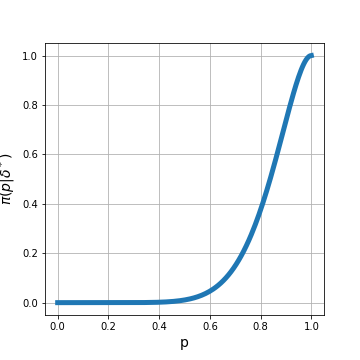
\includegraphics[scale=1]{power.png}
	%	\caption{Função Poder c = 8}
	%	\label{fig:power}
	\end{center}
	
	
\end{enumerate}
	
	
	\mysection{5}{Testes Randomizados} (Bônus) Mostre que, no item anterior, não é possível atingir qualquer nível $\alpha_0$, isto é, que $\alpha_0$ toma um número finito de valores.
	Proponha uma solução para que seja possível atingir qualquer nível em $(0, 1)$.
	
	\textbf{Solução:}
	\citep{degroot2012probability_random} Como vimos pela tabela, o fato da distribuição binomial ser discreta, impede que seja possível atingir qualquer $\alpha_0$. Uma solução alternativa, soluciona isso facilmente:
	
	No teste modificado, se $y<c$, rejeita-se $H_0$, se $y>c$ falha-se em rejeitar $H_0$, mas se $y=c$, rejeitamos $H_0$ com probabilidade $q$ de tal forma que:
	
	$\pr(y>c|p=1/2)+q\pr(y=c|p=1/2)=\alpha_0$
	
	Assim, fazendo $q=\dfrac{\alpha_0-\pr(y>c|p=1/2)}{\pr(y=c|p=1/2)}$ chegamos ao nível desejado.
	
	No caso acima, com c = 8, $\alpha_0=0.05$, temos $q=0.89\overline{3}$ (Python 3.7).
	
	
	
	
	
	
	
	
	
	
	
	\newpage
	%\printbibliography
	 \bibliographystyle{plain}
	 \bibliography{refs}
	
\end{document}        